\documentclass[a4paper]{article}

\usepackage[brazilian]{babel}
\usepackage[utf8]{inputenc}
\usepackage[T1]{fontenc}
\usepackage{lipsum}
\usepackage{todonotes}
\usepackage{natbib}
\usepackage{booktabs}
\usepackage{graphicx}

\title{Aplicação de mineração de dados ao problema de evasão de estudantes da UFC}

\author{Abelardo Vieira Mota}

\date{\today}

\begin{document}
\maketitle

\begin{abstract}
resumo
\end{abstract}

\tableofcontents

\section{Introdução}

\subsection{Contextualização}
\todo{necessidade, tendência}
O Programa de Apoio a Planos de Reestruturação e Expansão das Universidades Federais(REUNI) foi instituído pelo DECRETO Nº 6.096, DE 24 DE ABRIL DE 2007 \todo{como cita isso?} possui como uma de suas diretrizes:
\begin{quote}
I - redução das taxas de evasão, ocupação de vagas ociosas e aumento de vagas de ingresso, especialmente no período noturno;
\end{quote}
\todo{DECRETO Nº 6.096, DE 24 DE ABRIL DE 2007}

\todo{na ufc}
Na UFC, de acordo com o último Anuário estatístico\todo{quando sai o próximo?}, de 2014, ano base 2013, o indicador "Taxa de Sucesso na Graduação"(TS) \todo{figura}, definido como a proporção entre número de diplomados e número de ingressantes da graduação, esteve em 2013 com o menor valor desde que passou a ser monitorado. Já o indicador "Taxa de sucesso da graduação por curso", em 2013\todo{qual a definição?}, possuiu valor médio igual a 64\% e mínimo de 11.7\% para o curso Letras Português-Alemão, considerando a média entre os anos 2013, 2012 e 2011, para os cursos que tiveram valores calculados nesses anos.
\todo{dados do anuário mais detalhados}

\todo{como resolve}
Uma das estratégias para diminuir as taxas de evasão é a identificação precoce de estudantes com grande tendência para abandonarem seus cursos e a execução de ações que minimizem tal tendência. A identificação pode ser conduzida por observação do comportamento e resultados dos alunos, de forma subjetiva, pelos docentes e coordenadores de cursos, por exemplo. Dois problemas decorrer dessa forma de identificação: sendo conduzida por pessoas, essa forma de identificação é limitada pelo conjunto de observações as quais o observador tem acesso; sendo subjetiva, seus resultados podem sofrer resistência para serem aceitos. A utilização de técnicas de mineração de dados como forma de identificação pode contornar esses problemas por, primeiro, fazer uso de dados registrados por sistemas de informação, provavelmente contendo informações mais amplas que as que uma docente, por exemplo, pode observar; segundo, por fazer maior uso de dados registrados, sendo aceita mais facilmente como identificação objetiva. Dessa forma, podem colaborar com a solução do problema, seja auxiliando na identificação por pessoas, seja realizando a identificação automaticamente.

\todo{dados na ufc}
Os dados gerenciados pelos sistemas de informação da UFC podem conter informações que auxiliem o entendimento das causas desse problema e permitam que melhor sejam planejadas ações para solucioná-lo ou que estudantes com maior risco de evasão sejam identificados e recebam apoio da instituição. É nesse sentido, que a área de pesquisa denominada mineração de dados(data mining, em inglês), que estuda como extrair informações sobre dados, pode contribuir, fornecendo meios para a descoberta de informações relevantes a partir dos dados registrados pela UFC.

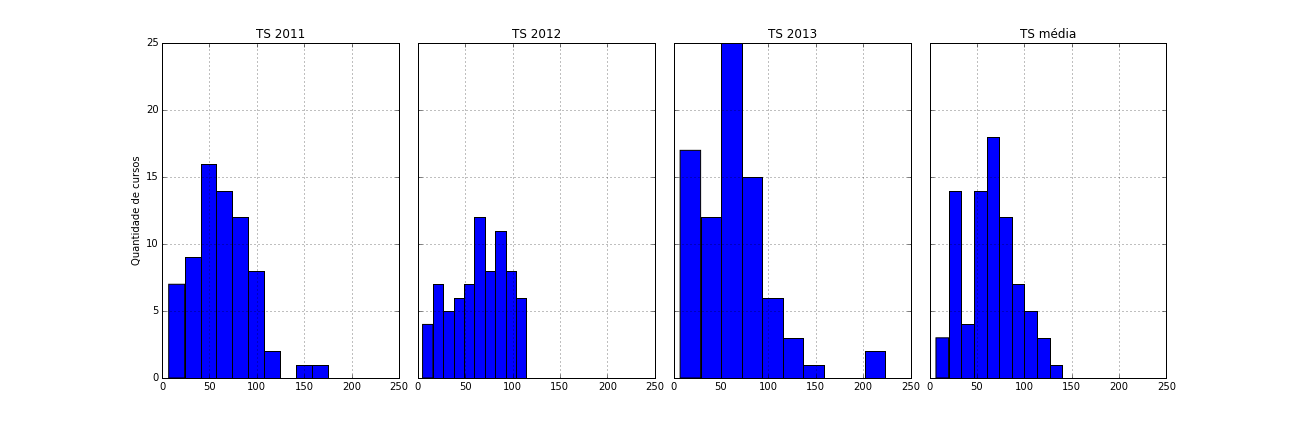
\includegraphics[scale=0.4, trim=60mm 0mm 0mm 0mm]{taxa-de-sucesso-ufc-hist}


\todo{falar sobre os estudos sobre drop-out+data mining}

\subsection{Objetivos}
O presente trabalho objetiva avaliar a aplicabilidade de técnicas de mineração de dados sobre o problema de evasão de estudantes na UFC a partir dos dados que seus sistemas de informação gerenciam.  

Para tanto é necessário que seja feito uma análise sobre a estrutura e qualidade dos dados disponíveis.

Também serão levantadas hipóteses sobre causas para o problema e será analisado se os dados as corroboram ou não.

hipótese sobre a estrutura do curriculo -> métricas com relação às turmas! por exemplo, distância de horário entre disciplinas do mesmo semestre -> no caso do aluno, para cada semestre calcular

\subsection{Organização do trabalho}
\todo{no fim}
\section{Mineração de dados}
\todo{sobre data mining - qual o super artigo básico?}
\subsection{Identificação de padrões}
\todo{clustering, visualização}
\subsection{Aprendizado de máquina}
De acordo com \cite{Tom_mitchell} \todo{como por a definition?}

Definition: A computer program is said to learn from experience E with respect to some class of tasks T and performance measure P, if its performance at tasks in T, as measured by P, improves with experience E. 
\todo{bla bla bla de machine learning}

\todo{definição informal de aprendizado de máquina}
\todo{definição formal de aprendizado de máquina}
\todo{métricas}
\todo{algoritmos}
\todo{métodos de teste}
\cite{ML_debt} \cite{ML_know}
\todo{machine learning}
\bibliographystyle{plain}

\section{Evasão de estudantes}
\todo{tabela com dados dos estudos analisados - ver fichamento.xlsx}
\todo{descrever, em termos gerais, cada estudo}
Em \cite{EDM_pred_dropout} são aplicados algoritmos de aprendizado de máquina a dados de estudantes do Eletrical Engineering department, Eindhoven University of Technology , com o objetivo de identificar estudantes em grupos de risco de evasão. É relatado que esse departamento já avaliava os estudantes com relação ao risco de evasão, mas de forma subjetiva. O estudo ressalta o maior custo da ocorrência de falsos negativos que de falsos positivos na identificação de estudantes com risco de evasão. Ocorre que, argumenta-se, há prejuízo maior em não oferecer apoio a um estudante com risco de evasão do que oferecer, desnecessariamente, apoio a um estudante sem tal risco. O estudo faz uso então de uma matriz de custo, com o classificador CostSensitiveClassifier, do Weka, obtendo melhores resultados, com relação a ocorrência de falsos negativos, mas com perdas de acurácia. 

\cite{EDM_review_and_soa} 
\cite{EDM_retention} 
\cite{EDM_education}
\cite{EDM_dropout_rates}
\cite{EDM_ufrj}
\cite{EDM_ufrj2}
\cite{EDM_brasil}

\bibliography{dissertacao}

\end{document}